\documentclass[10pt,pdftex,a4paper,twoside,openright]{book}

\usepackage[hmarginratio=3:2, vmargin=1in]{geometry}

%German setting
\usepackage{ngerman}
\usepackage[latin1]{inputenc}
\usepackage[official]{eurosym}
\usepackage[T1]{fontenc}

\usepackage{graphicx}  % Include grafics
\usepackage{grffile}   % support special grafic names
\usepackage{listings}  % Source code

\usepackage{listings}
\usepackage{pdf}
\usepackage{titleref}  % Referenz with name
\usepackage{wrapfig}


\pagestyle{fancy}
% Links nur Kapitel (Gro�keinschreibung statt alles Gro�)
\fancyhead[L]{\nouppercase{\leftmark}}
% Rechts nichts
\fancyhead[R]{}

\setcounter{tocdepth}{3}
\setcounter{secnumdepth}{3} 

\providecommand{\versionnumber}{19.10}


\title{Raspberry Pi Jam - Raspjamming\\Installation/Vorbereitung/Microsoft Windows}
\author{\textbf{Autoren:}\\
	Martin Strohmayer\\
	Christoph W�rg�tter\\
	Christof Hirndler\\
	Manfred Wallner\\
}
\date{Version \versionnumber \\\today \\PDF Edition}

\begin{document}

\maketitle

\tableofcontents

\chapter{Installation Raspberry Pi}

\section{Raspbian}


Raspbian ist das offizielle Betriebssystem f�r den Raspberry~Pi. F�r die Verwendung bei einem Raspberry Pi Jam wurde ein eigenen Image vom Grazer Computer Club (GC2) mit dem Namen Raspjamming erstellt und zur Verf�gung gestellt. Ausgehend vom 
Raspbian Lite Image wurde noch verschiedene Entwickerlerprogramm und Werkzeuge installiert. Zus�tzlich wurde das System so eingerichtet, dass die Raspberry Pi Zero direkt �ber den USB-OTG Anschluss mit dem Host PC verbunden werden kann. Der SSH-Dienst und WLAN wurde aktiviert. Alle L�ndereinstellung wurden  von UK auf �sterreich/German ge�ndert. Ein Web-Server stellt Programme und Hilfe zur Verf�gung, auch ohne Internet..\\  
F�r die Installation ben�tigt man ein beliebiges Linux System mit einem MicroSD-Kartenleseger�t.  Es wird mindestens eine 4~GB gro�e MicroSD-Karte ben�tigt. Die aktuelle Raspjamming Version kann als Image-Datei von der Seite \url{https://github.com/GrazerComputerClub/Raspjamming-Image} heruntergeladen werden. 

\begin{console}
	wget --trust-server-names http://www.strohmayers.com/image/2019-02-07-Raspjamming-full.zip
	unzip 2019-02-07-Raspjamming-full.zip
	rm 2019-02-07-Raspjamming-full.zip
\end{console}


\subsection{Etcher}

Das grafische Programm Etcher (\url{https://etcher.io}) kann zum �bertragen der Image-Datei verwendet werden. Es ist vor Allem f�r Anf�nger zu empfehlen, da beim Konsolenprogramm dd das Risiko besteht, dass Daten einer falschen Partition bzw. eines Laufwerks zerst�rt werden. Das Programm muss allerdings manuell installiert werden.     

\begin{console}
	wget https://github.com/resin-io/etcher/releases/download/v1.3.1/etcher-1.3.1-linux-x86_64.zip 
	unzip etcher-1.3.1-linux-x86_64.zip
	chmod +x etcher-1.3.1-x86_64.AppImage
	sudo mv etcher-1.3.1-x86_64.AppImage /usr/local/bin/etcher
	etcher &
\end{console}


Nach dem Starten wird danach gefragt ob eine Verkn�pfung zum Programm erstellt werden soll. Dies sollte man mit "`Yes"' beantworten. Danach kann man mit der Schaltfl�che "`Image"' die Image-Datei ausw�hlen. Ist nur ein m�gliches Ziel vorhanden, wird es bereits vorausgew�hlt, z.~B. die SD-Karte im Karten-Slot (/dev/memcblk0) oder im USB-Adapter (/dev/sdb). Sind mehrere m�gliche Ziele vorhanden, wird die "`Select Drive"' Schaltfl�che freigeschaltet. Dann kann ein Laufwerk manuell ausgew�hlt werden.

\begin{figure}[ht]
	\centering
	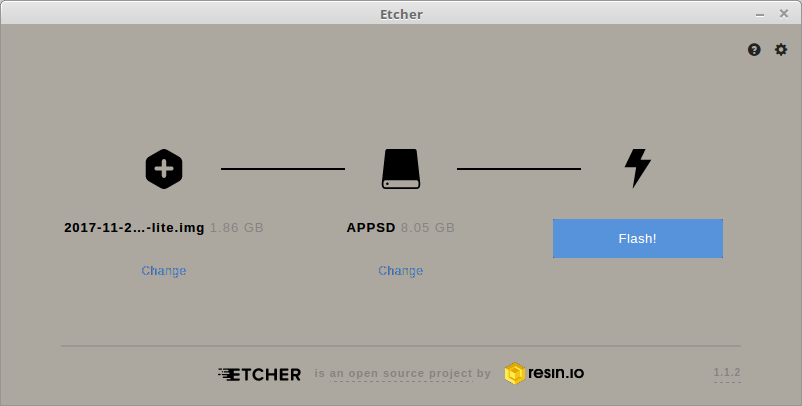
\includegraphics[scale=0.3]{images/Etcher_1.png}
	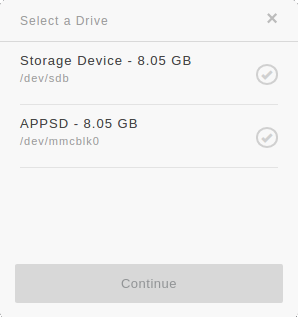
\includegraphics[scale=0.3]{images/Etcher_2.png}
	\label{Etcher}
\end{figure}


Wenn man noch etwas �ndern will, kann die entsprechende "`Change"' Schaltfl�che ausgew�hlt werden. Zum Schluss wird der Schreibvorgang mit der "`Flash!"' Schaltfl�che gestartet. M�glicherweise wird vom Programm allerdings noch das System-Passwort abgefragt.\\ 
Das Laufwerk bzw. die Partitionen werden nun aus dem System ausgeh�ngt und der Schreibvorgang gestartet. Der Fortschritt, die durchschnittliche �bertragungsrate und die Restlaufzeit werden w�hrend des Vorgangs angezeigt.\\ 


\subsection{dd Kommandozeilenprogramm}

Die erhaltene Image-Datei kann mit dem Kommandozeilenprogramm dd auf eine MicroSD-Karte �bertragen werden.\\
\textbf{Es ist unbedingt vor dem Ausf�hren des Befehls zu pr�fen, ob das angegebene Laufwerk bzw. Device auch der vorgesehenen MicroSD-Karte entspricht!}\\ 
Bei USB-Kartenlesern bzw. USB-Adaptern ist die Ermittlung des Devices leicht �ber die Systemmeldungen m�glich. 

\begin{console}
	dmesg | tail -n 10
\end{console}

\begin{screensmall}
	scsi 3:0:0:0: Direct-Access     MXT-USB  Storage Device   1308 PQ: 0 ANSI: 0 CCS
	sd 3:0:0:0: Attached scsi generic sg1 type 0
	sd 3:0:0:0: [sdb] 15730688 512-byte logical blocks: (8.05 GB/7.50 GiB)
	sd 3:0:0:0: [sdb] Write Protect is off
	sd 3:0:0:0: [sdb] Mode Sense: 03 00 00 00
	sd 3:0:0:0: [sdb] No Caching mode page found
	sd 3:0:0:0: [sdb] Assuming drive cache: write through
	sdb: sdb1 sdb2
	sd 3:0:0:0: [sdb] Attached SCSI removable disk
	EXT4-fs (sdb2): mounted filesystem with ordered data mode. Opts: (null)
\end{screensmall}

Die MicroSD-Karte wurde im Beispiel als Device "`sdb"' �ber einen USB-Adapter eingebunden. Nun kann man die Image-Datei mit dem Programm dd auf die MicroSD-Karte �bertragen. Mit dem Parameter "`of"' muss der komplette Device-Name, in diesem Fall "`/dev/sdb"', angegeben werden. Bei Parameter "`if"' wird die entpackte Image-Datei angeben. Die Bl�ckgr��e bzw. der Cache wird mit Parameter "`bs"' gesetzt. Eine gr��ere Blockgr��e erh�ht die Schreibgeschwindigkeit. Sie wird im Beispiel mit 4~MB angegeben.\\
Zu Beachten ist, dass der USB-Massenspeicher m�glicherweise bereits automatisch gemountet wurde. Dann sollte man die Partitionen mit dem Befehl "`umount"' zuerst auswerfen. 


\begin{console}
	umount /dev/sdb1 /dev/sdb2
	dd if=2019-02-07-Raspjamming-full.img of=/dev/sdc bs=4M
\end{console}

\begin{screensmall}
	2623+0 Datens�tze ein
	2623+0 Datens�tze aus
	2387266048 Bytes (2,4 GB) kopiert, 247,6147 s, 10,4 MB/s
\end{screensmall}



\section{USB Gadget / OTG Mode ZeroConf (Raspberry Pi Zero)}


Beim USB-Gadget oder OTG-Betrieb kann die Raspberry Pi Zero direkt �ber den Micro-USB-Anschluss mit einem PC oder Laptop verbunden werden. Er verh�lt sich dann wie ein USB-Ger�t und kann z.~B. ein Massenspeicher-, Serielles-  oder Netzwerkger�t simulieren.\\
Verh�lt er sich als Netzwerkger�t kann eine Netzwerkverbindung �ber ein virtuelles Netzwerk zum Ger�t hergestellt werden. 
Weitere Informationen �ber den OTG-Betrieb kann der Git-Hub Seite  \url{https://gist.github.com/gbaman/50b6cca61dd1c3f88f41} entnommen werden.

\subsection{Client - Raspberry Pi Zero}

Nach der Einrichtung des Betriebssystems auf der MicroSD-Karte m�ssen noch ein paar Modifikationen an den Dateien der Boot-Partition durchgef�hrt werden. 

Folgender Text muss nach der Anweisung "`rootwait"' in die Datei "`cmdline.txt"' eingef�gt werden:
\begin{screensmall}
modules-load=dwc2,g_ether g_ether.host_addr=00:01:02:03:04:05 g_ether.dev_addr=00:01:02:03:04:06
\end{screensmall}

Die Angabe der MAC-Adresse f�r Host und Ger�t ist optional, es wird aber empfohlen da sonst diese Adressen zuf�llig vergeben werden. Die Werte k�nnen frei gew�hlt werden, sollten sich aber nicht mit den Adressen im Netz bzw. Host �berschneiden.\\

Folgende Zeile muss am Ende in die Datei "`config.txt"' hinzugef�gt werden:
\begin{screensmall} 
dtoverlay=dwc2
\end{screensmall}

Weiters muss eine leere Datei mit dem Namen "`ssh"' erzeugt werden, damit der SSH-Dienst automatisch nach dem Start ausgef�hrt wird. Danach kann die MicroSD-Karte in den Raspberry Pi Zero gesteckt und �ber ein MicroUSB-Kabel an einen Computer angeschlossen werden. 
Es ist zu beachten, dass das MicroUSB-Kabel am mittleren MicroUSB-Anschluss angeschlossen werden muss!\\

%\begin{console} 
%	touch /mnt/ssh
%\end{console} 

%Wird Microsoft Windows verwendet so muss das Programm Bonjour von Apple installiert werden. 
%Falls der Dienst noch nicht von einem Apple Programm (iTunes oder Quicktime) installiert wurde, kann von der Seite \url{https://support.apple.com/kb/DL999?locale=de_AT} ein Setup heruntergeladen werden.\\

\input{OTG_Kubuntu_ZeroConf}

\input{OTG_Internet}

Sp�ter wird noch die IP-Adresse der lokalen Raspberry Pi Verbindung ben�tigt. Dies ermittelt man in der Konsole mit dem Befehl \texttt{ifconfig}.  

\begin{console} 
	ifconfig enx000102030405 | head -n 2
\end{console}

\begin{screensmall} 
	enx000102030405 Link encap:Ethernet  Hardware Adresse 00:01:02:03:04:05  
	inet Adresse:169.254.144.15  Bcast:169.254.255.255  Maske:255.255.0.0
\end{screensmall}





Nach der Einrichtung kann per SSH-Client eine Verbindungen zum Raspberry Pi hergestellt werden. Dazu muss in einem Terminal folgender Befehl eingegeben werden:

\begin{console} 
	ssh -X pi@raspberrypi.local
\end{console}

Um grafische Programme am Host anzeigen zu k�nnen, muss der Parameter \texttt{-X} angegeben werden. "`\textbf{pi}"' ist der Standardbenutzer am System. Dann wird eine X-Server Verbindung via SSH hergestellt. Verbindet man sich zum ersten Mal mit dem Raspberry Pi, so wird noch eine Sicherheitswarnung ausgegeben. Der kryptographische Schl�ssel f�r die Verbindung ist dem lokalen System noch nicht bekannt.%  und muss best�tigt werden.
\begin{screensmall}
The authenticity of host 'raspberrypi.local (192.168.137.10)' can't be established.
ECDSA key fingerprint is SHA256:Dcf3HYgE2GHnNnZ8Xhv8iJ9yA+zvfXBC9COm2eL9i0w.
Are you sure you want to continue connecting (yes/no)? 
Warning: Permanently added 'raspberrypi.local,192.168.137.10' (ECDSA) to the list of known hosts.
\end{screensmall}

Die Frage muss mit \texttt{yes} best�tigt werden. Anschlie�end muss das Default-Passwort von Raspbian "`\textbf{raspberry}"' eingegeben werden. Nun sollte man den Raspberry Pi Prompt \texttt{pi@rasbperrypi:\textasciitilde  \$} sehen. 

Wechselt man zu einem anderen Raspberry Pi mit den gleichen Namen oder installiert das System nochmals, so kann es passieren, dass eine Fehlermeldung ausgegeben wird, weil sich der kryptographische Schl�ssel ge�ndert hat.

\begin{screensmall} 
@@@@@@@@@@@@@@@@@@@@@@@@@@@@@@@@@@@@@@@@@@@@@@@@@@@@@@@@@@@
@    WARNING: REMOTE HOST IDENTIFICATION HAS CHANGED!     @
@@@@@@@@@@@@@@@@@@@@@@@@@@@@@@@@@@@@@@@@@@@@@@@@@@@@@@@@@@@
\end{screensmall} 

%The ECDSA host key for raspberrypi.local has changed,
%and the key for the corresponding IP address 169.254.229.192
%is unknown. This could either mean that
%DNS SPOOFING is happening or the IP address for the host
%and its host key have changed at the same time.
%@@@@@@@@@@@@@@@@@@@@@@@@@@@@@@@@@@@@@@@@@@@@@@@@@@@@@@@@@@@
%@    WARNING: REMOTE HOST IDENTIFICATION HAS CHANGED!     @
%@@@@@@@@@@@@@@@@@@@@@@@@@@@@@@@@@@@@@@@@@@@@@@@@@@@@@@@@@@@
%IT IS POSSIBLE THAT SOMEONE IS DOING SOMETHING NASTY!
%Someone could be eavesdropping on you right now (man-in-the-middle attack)!
%It is also possible that a host key has just been changed.
%The fingerprint for the ECDSA key sent by the remote host is
%SHA256:Dcf2HYyE2GHnNpZ8Xhv8iJ9yj+zvfXBC9COm2eL9i0w.
%Please contact your system administrator.
%Add correct host key in /home/evil/.ssh/known_hosts to get rid of this message.
%Offending ECDSA key in /home/evil/.ssh/known_hosts:9
%remove with:
%ssh-keygen -f "/home/evil/.ssh/known_hosts" -R raspberrypi.local
%ECDSA host key for raspberrypi.local has changed and you have requested strict checking.

In diesem Fall muss man die Verbindung aus den bekannten Hosts l�schen. Hierf�r muss folgendes Kommando ausgef�hrt werden:

\begin{console} 
	ssh-keygen -R raspberrypi.local
\end{console}

Optional kann auch der Parameter \texttt{-o UserKnownHostsFile=/dev/null} beim ssh-Befehl hinzugef�gt werden. Dann erfolgt keine �berpr�fung der Verbindung. 

~\\
Nun muss noch der Gateway am Client eingestellt werden. Dazu muss die IP-Adresse des Host-PC bekannt sein. Im Beispiel muss die IP-Adresse "`169.254.144.15"' durch die IP-Adresse des Hosts ersetzt werden.   


\begin{console} 
	sudo route add default gw 169.254.144.15
\end{console}

\clearpage
\section{USB Gadget / OTG Mode DHCP-Server (Raspberry Pi Zero)}

\begin{figure}[ht]
	\centering
	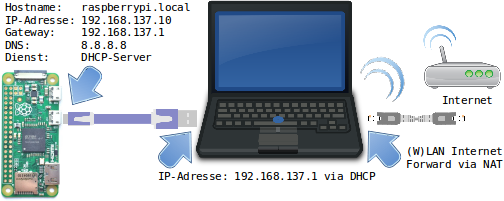
\includegraphics[scale=0.84]{images/Aufbau_Schema.png}
	%	\label{Aufbau_Schema}
\end{figure}

\subsection{Client - Statische IP-Adresse und DHCP Server}

Die folgende Einstellungen m�ssen nicht gemacht werden, erleichtern aber das Arbeiten. Der Raspberry Pi Zero hat dann eine statische IP-Adresse und kann leichter angesprochen und auch die Internetverbindung freigegeben werden (vor allem mit Microsoft Windows 7 und 10).\\
Am Client-System, also der Raspberry Pi Zero, kann die Netzwerkadresse, der Gateway und ein DNS-Server eingestellt werden. Dieser Schritt ist unbedingt n�tig wenn die Internetverbindung unter Windows dem Ger�t zur Verf�gung gestellt werden soll. Die IP-Adresse die eingestellt wird, muss f�r Windows 7 aus dem Bereich 192.168.137.* sein (z.~B. 192.168.137.10). Der Gateway ist die IP-Adresse des Host-PC. Als DNS-Server kann z.~B. der Server von Google mit der Adresse 8.8.8.8 verwendet werden. Die Einstellungen k�nnen in der Konfigurationsdatei f�r den DHCP-Client definiert werden.\\ 
Die IP-Adresse des Host-Computers kann via eines DHCP-Server konfiguriert werden. Das hat den Vorteil, dass dort keine Konfiguration des Netzwerks erfolgen muss. Es wird zur weiteren Einrichtung ein Terminalzugang zum Einplatinencomputer ben�tigt und eine Internetverbindung sollte bestehen damit man den DHCP-Server installieren kann.\\
Per SSH-Client kann eine Verbindungen zum Raspberry Pi mit dem Befehl "'ssh pi@raspberrypi.local"' hergestellt werden. %Nun kann die Konfiguration abgeschlossen werden.   

\begin{console}
	sudo vi /etc/dhcpcd.conf
\end{console}

Folgende Zeilen m�ssen am Ende der Datei eingef�gt werden:\\

\filename{/etc/dhcpcd.conf [-rw-r-{-}r-{-} root root]}
\begin{file}
	
# define static profile for Pi 
profile static_usb0
static ip_address=192.168.137.10/24
static routers=192.168.137.1
static domain_name_servers=8.8.8.8

# static profile on usb0
interface usb0 
fallback static_usb0
\end{file}


\begin{console}
	sudo apt-get update
	sudo apt-get install isc-dhcp-server
\end{console}

%Falls die Internetverbindung am Raspberry Pi Zero nicht m�glich ist, kann der Server auch manuell heruntergeladen, auf der Boot-Partition gespeichert und installiert werden.\\
%Install-Datei:
%\url{http://archive.raspbian.org/raspbian/pool/main/i/isc-dhcp/isc-dhcp-server_4.3.5-3_armhf.deb}
%	
%	\begin{console}
%		sudo dpkg -i /boot/isc-dhcp-server_4.3.1-6+deb8u2_armhf.deb
%	\end{console}
%	
%	Nach der Installation kann der DHCP-Server parametriert werden. 
	
\begin{console}
	sudo vi /etc/dhcp/dhcpd.conf
\end{console}

%ddns-update-style none;

%#option domain-name "example.org";
%#option domain-name-servers ns1.example.org, ns2.example.org;

%default-lease-time 600;
%max-lease-time 7200;
%
%log-facility local7;


Folgende Zeilen m�ssen am Ende der Datei eingef�gt werden:\\

\filename{/etc/dhcp/dhcpd.conf [-rw-r-{-}r-{-} root root]}
\begin{file}
subnet 192.168.137.0 netmask 255.255.255.0{
	range 192.168.137.2 192.168.137.9;
	option broadcast-address 192.168.137.255;
}

#USB OTG Host-PC set IP-Address to 192.168.137.1
host USB_OTG_HOST {
	hardware ethernet 00:01:02:03:04:05;
	fixed-address 192.168.137.1;
}
\end{file}

\begin{console}
	sudo reboot
\end{console}


\subsection{Host (DHCP-Client)}

\subsubsection{Windows 7}

Nach dem Boot wird automatisch ein neues "`RNDIS/Ethernet Gadget"' erkannt und Treiber installiert. Sollte die Installation nicht erfolgreich abgeschlossen werden k�nnen, so muss man den Treiber manuell installieren.

\begin{figure}[ht]
  \centering
  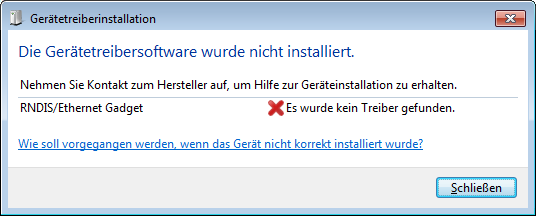
\includegraphics[scale=0.42]{images/OTG_Win7_InstallFail.png}
%  \caption{Windows Treiber konnte nicht automatisch installiert werden}
  \label{OTG_Win7_InstallFail}
\end{figure}

\begin{figure}[ht]
  \centering
  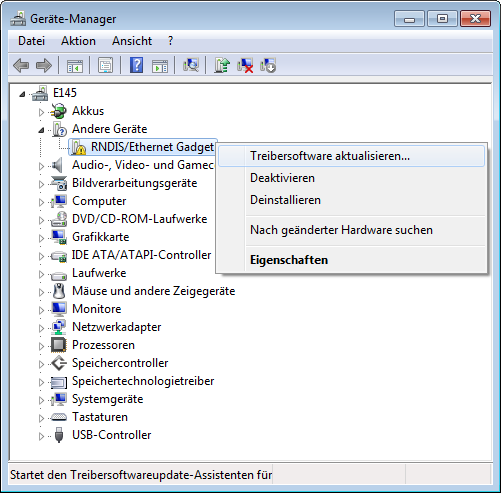
\includegraphics[scale=0.42]{images/Geraetemanager.png}
%  \caption{Windows Treiber konnte nicht automatisch installiert werden}
  \label{OTG_Win7_InstallManual}
\end{figure}

%Dazu �ffnet man den Gr�temanager, aktiviert das fehlerhafte Ger�t unter "`Andere Ger�te"' und �ffnet mit der rechten Maustaste das Kontextmen�. 
Dazu �ffnet man zuerst den Gr�temanager. Dann �ffnet man das Kontextmen� in dem man die rechten Maustatste am 
fehlerhaften Ger�t (Andere Ger�te / RNDIS/Ethernet Gadget) dr�ckt. Nun w�hlt man den Men�punkt "`Treiber Software aktualisieren..."' aus. Im folgenden Dialog w�hlt man "`Auf dem Computer nach Treibersoftware suchen"' und dann "`Aus einer Liste von Ger�tetreibern auf dem Computer ausw�hlen"'. Danach kann der Ger�tetyp gew�hlt werden in dem man "`Netzwerkadapter"' ausw�hlt. Dann w�hlt man den Hersteller "`Microsoft Corporation"' und den Netzwerkadapter "`Remote NDIS based Internet Sharing Device"'. Sollte eine Kompatibilit�tswarnung angezeigt werden, kann der Treiber trotzdem installiert werden. Zum Schluss sollte der Treiber automatisch erfolgreich installiert werden.\\ 

\begin{figure}[ht]
  \centering
  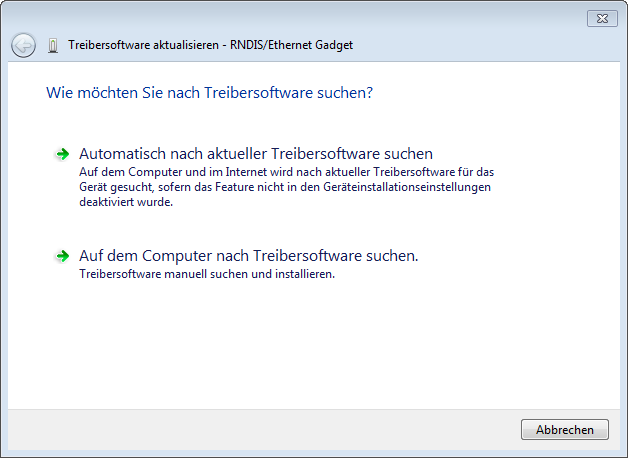
\includegraphics[scale=0.42]{images/OTG_Win7_Install_1.png}
	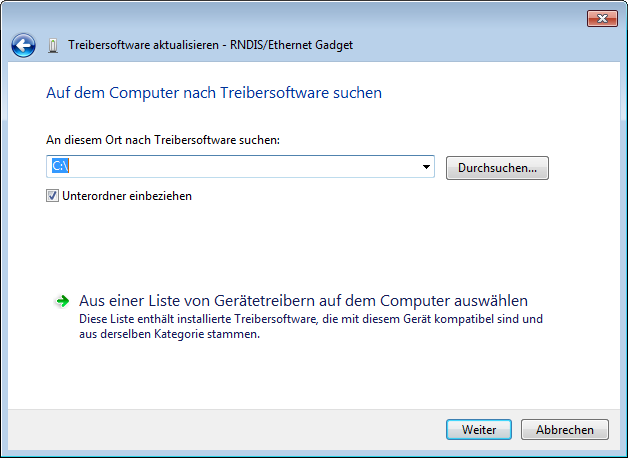
\includegraphics[scale=0.42]{images/OTG_Win7_Install_2.png}
 
%  \caption{}
  \label{OTG_Win7_Install_12}
\end{figure}

\begin{figure}[ht]
  \centering
  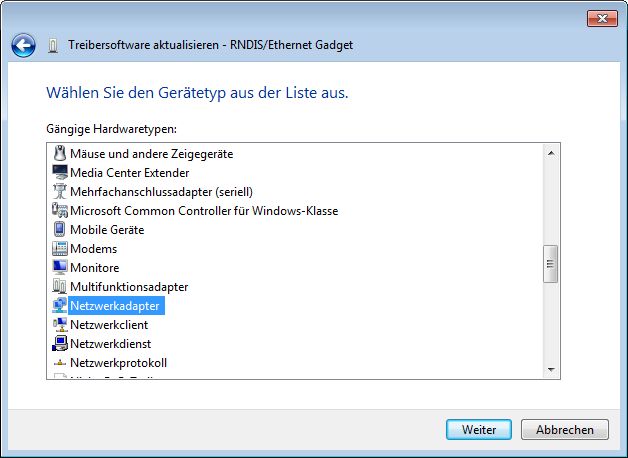
\includegraphics[scale=0.42]{images/OTG_Win7_Install_3.png}
  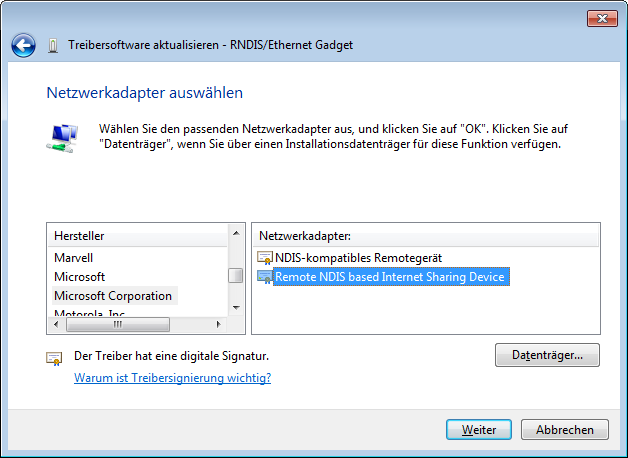
\includegraphics[scale=0.42]{images/OTG_Win7_Install_4.png}
%  \caption{}
  \label{OTG_Win7_Install_34}
\end{figure}


\begin{figure}[ht]
  \centering
  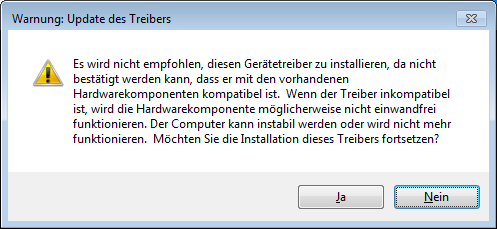
\includegraphics[scale=0.50]{images/OTG_Win7_Install_5.png}
  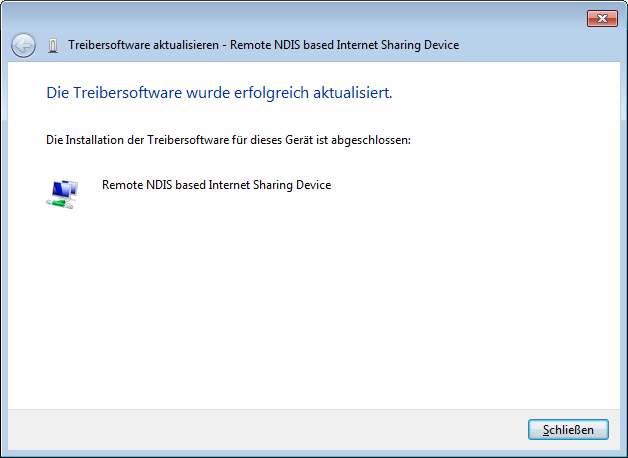
\includegraphics[scale=0.42]{images/OTG_Win7_Install_6.png}
%	\caption{}
  \label{OTG_Win7_Install_56}
\end{figure}


Damit am Ger�t Internet funktionieren kann, muss das Internet f�r das neue Netzwerk freigegeben werden. Dazu �ffnet man das Einstellungs-Fenster f�r die Netzwerkverbindungen. 

\begin{figure}[ht]
  \centering
  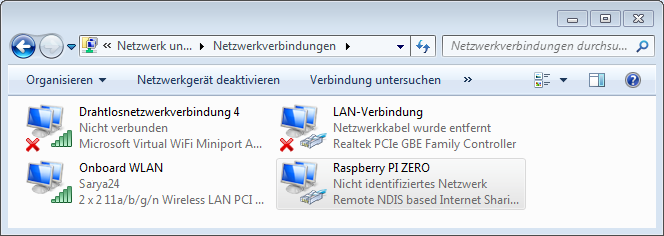
\includegraphics[scale=0.42]{images/OTG_Win7_Netzwerkverbindungen.png}
%	\caption{}
  \label{OTG_Win7_Netzwerkverbindungen}
\end{figure}

Zuerst kann man dem Netzwerkger�t "`Remote NDIS based Internet Sharing Device"' einen neuen Namen geben, z.~B. Raspberry PI ZERO. Nun muss das Netzwerk gesucht werden, das mit dem Internet verbunden ist, z.~B. Onboard WLAN. Bei den Eigenschaften zu dem Netzwerk kann der Reiter "`Freigabe"' ausgew�hlt werden. Danach kann man die Einstellung "`Anderen Benutzern im Netzwerk gestatten, diese Verbindung des Computers als Internetverbindung zu verwenden"' aktivieren und bei Heimnetzwerkverbindung kann das Netzwerk "`Raspberry PI ZERO"' ausgew�hlt werden.\\
Windows 7 legt dann fest, dass die Netzwerkadresse 192.168.137.1 sein muss. Alternativ kann die Verbindung auch zuvor schon auf diese statische IP-Adresse gesetzt werden.\\



\begin{figure}[ht]
  \centering
  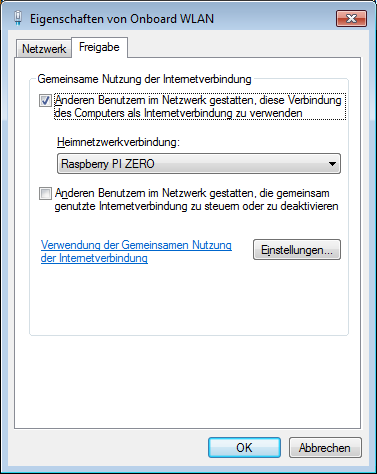
\includegraphics[scale=0.42]{images/OTG_Win7_Inet.png}
  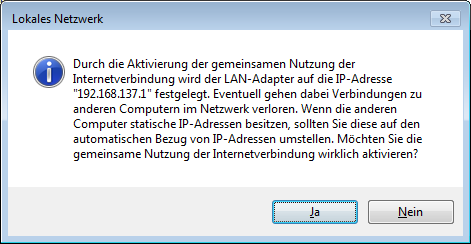
\includegraphics[scale=0.42]{images/OTG_Win7_Inet2.png}
%	\caption{}
  \label{OTG_Win7_Inet_12}
\end{figure}


Nun kann die Verbindung zur Raspberry Pi mit dem Programm Putty und der Adresse "`192.168.137.10"', �ber das SSH-Protokoll hergestellt werden.\\  
Mit dem Befehl "`ping 8.8.8.8"' kann die Internetverbindung getestet werden. Mit dem Befehl "`ping google.com"' kann dann der DNS-Server �berpr�ft werden.   


\clearpage
\subsection{Windows 10}

Nach dem Boot wird der Raspberry Pi Zero als "`Serielles USB-Ger�t"' erkannt und keine korrekten Treiber installiert. Dies muss manuell erfolgen. Dazu l�dt man sich zuerst den zertifizierten Treiber "`Acer Incorporated. - Other hardware - USB Ethernet-RNDIS Gadget"' von der Microsoft Homepage herunter \url{http://download.windowsupdate.com/msdownload/update/driver/drvs/2012/12/20342322_4b9970e3174b23b5cb2371af0837f939a71271ea.cab} bzw. \url{https://tinyurl.com/y6onwaax}. Die ben�tigten Dateien sind in der komprimierten CAB-Datei enthalten. Durch einen Doppelklick auf der Datei kann der Inhalt dargestellt werden. Mit der rechten Maustaste und dem Kontexmen� k�nnen die Dateien z.~B. nach \path{c:\Drivers\RNDIS\} extrahiert werden. 

\begin{figure}[ht]
  \centering
  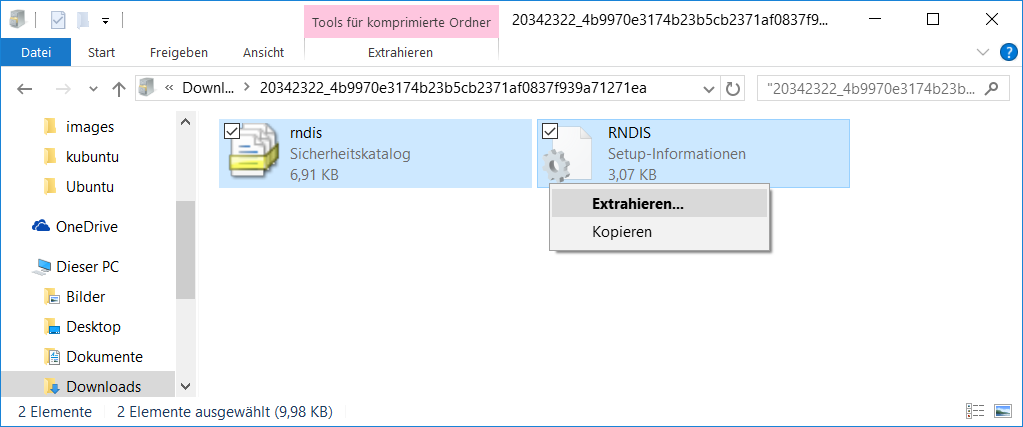
\includegraphics[scale=0.42]{images/OTG_Win10_Install_0.png}
%  \caption{}
  \label{OTG_Win10_Drivers}
\end{figure}

Nun muss der Gr�temanager ge�ffnet werden. Dann �ffnet man das Kontextmen� in dem man die rechte Maustaste am 
"`Serielles USB-Ger�t"' Eintrag dr�ckt. Nun w�hlt man den Men�punkt "`Treiber Software aktualisieren..."' aus. Im folgenden Dialog w�hlt man "`Auf dem Computer nach Treibersoftware suchen"' und dann gibt man das Verzeichnis an, in dem die Treiberdaten extrahiert wurden, z.~B. \path{c:\Drivers\RNDIS\}. Zum Schluss sollte der Treiber automatisch erfolgreich installiert werden.\\ 

\begin{figure}[ht]
  \centering
  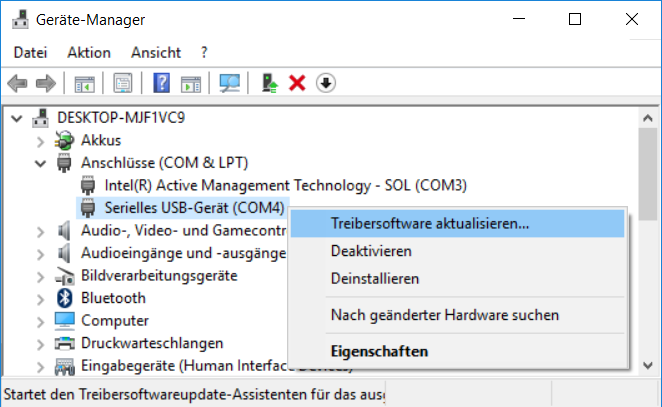
\includegraphics[scale=0.5]{images/OTG_Win10_Install_1.png}
  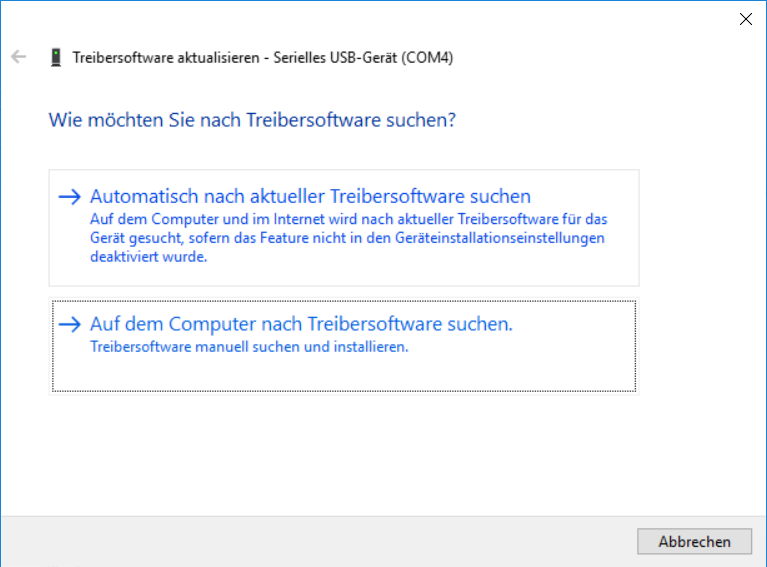
\includegraphics[scale=0.4]{images/OTG_Win10_Install_2.png}
%  \caption{}
  \label{OTG_Win10_Install_1}
\end{figure}


\begin{figure}[ht]
  \centering
  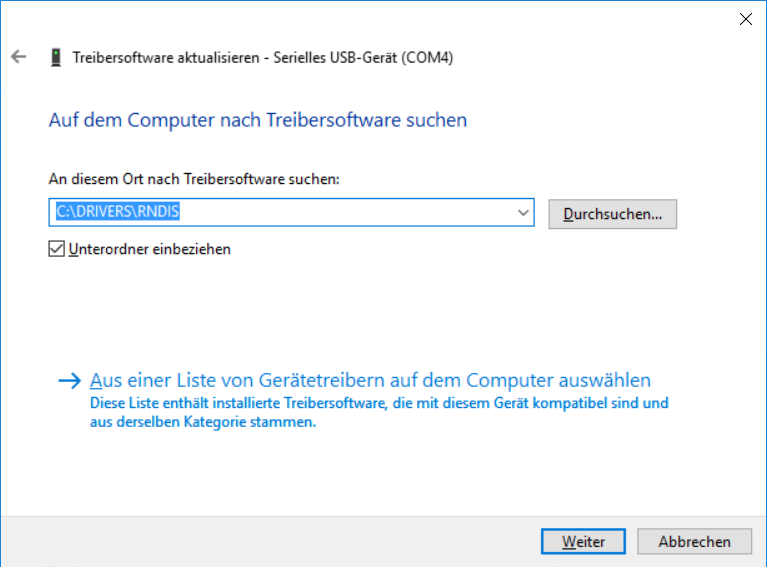
\includegraphics[scale=0.4]{images/OTG_Win10_Install_3.png}
  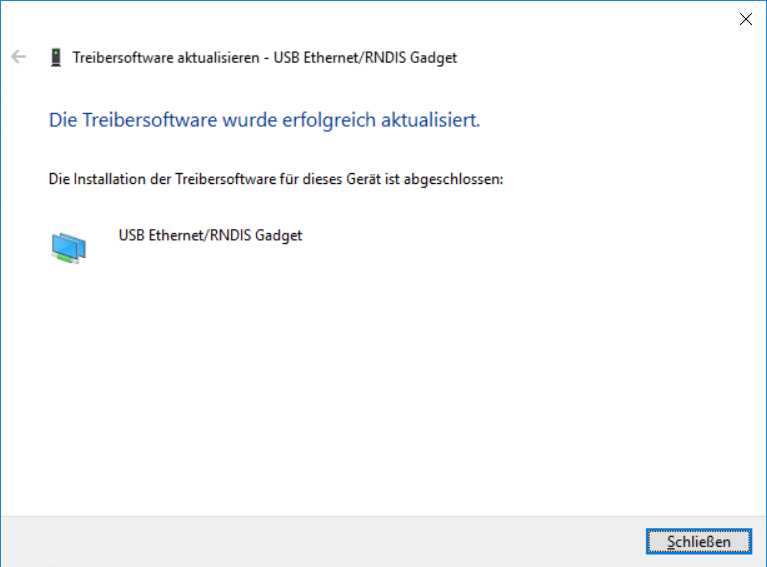
\includegraphics[scale=0.4]{images/OTG_Win10_Install_4.png}
%  \caption{}
  \label{OTG_Win10_Install_3}
\end{figure}  


Damit am Ger�t Internet funktionieren kann, muss das Internet f�r das neue Netzwerk freigegeben werden. Dazu �ffnet man das Einstellungs-Fenster f�r die Netzwerkverbindungen. 

\begin{figure}[ht]
  \centering
  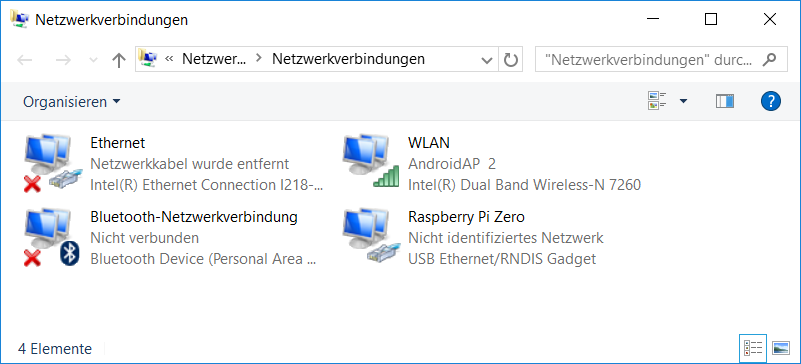
\includegraphics[scale=0.40]{images/OTG_Win10_Netzwerkverbindungen.png}
  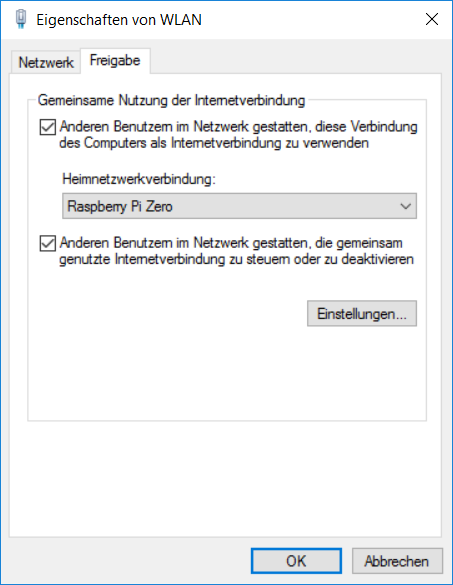
\includegraphics[scale=0.40]{images/OTG_Win10_Inet.png}
%	\caption{}
  \label{OTG_Win10_Netzwerkverbindungen}
\end{figure}

Zuerst kann man dem Netzwerkger�t "`USB Ethernet/RNDIS Gadget"' einen neuen Namen geben, z.~B. Raspberry Pi Zero. Nun muss das Netzwerk gesucht werden, das mit dem Internet verbunden ist, z.~B. WLAN. Bei den Eigenschaften zu dem Netzwerk kann der Reiter "`Freigabe"' ausgew�hlt werden. Danach kann man die Einstellung "`Anderen Benutzern im Netzwerk gestatten, diese Verbindung des Computers als Internetverbindung zu verwenden"' aktivieren und bei Heimnetzwerkverbindung kann das Netzwerk "`Raspberry Pi Zero"' ausgew�hlt werden.\\

Nun kann die Verbindung zur Raspberry Pi mit dem Programm Putty und der Adresse "`raspberrypi.local"', �ber das SSH-Protokoll hergestellt werden (siehe Kapitel \ref{sec:connection_putty} \titleref{sec:connection} - \titleref{sec:connection_putty}).\\  
Mit dem Befehl "`ping 8.8.8.8"' kann die Internetverbindung getestet werden. Mit dem Befehl "`ping google.com"' kann dann der DNS-Server �berpr�ft werden .   

\clearpage
\subsubsection{Kubuntu 16.04}

Am Host-PC muss bei den IPv4-Einstellungen die Methode "`Automatisch"' eingestellt sein. Wenn es sich um eine neue Verbindung handelt, ist dies bereits voreingestellt, eine Parametrierung kann dann entfallen. Ansonsten muss zur Konfiguration unter Linux (Kubuntu 16.04) zuerst der Dialog "`Netzwerkverbindungen"' ge�ffnet werden.\\ 
Dazu klickt man mit der rechten Maustaste auf das Netzwerksymbol in Infobereich rechts unten. Dann kann die Option "`Netzwerkverbindungen einrichten..."' ausgew�hlt werden.

\begin{figure}[ht]
  \centering
  
\includegraphics[scale=1.00]{images/OTG_NetzwerkverbindungenIcon.png}	
  
\includegraphics[scale=0.42]{images/OTG_NetzwerkverbindungenOpen.png}	
  %	\caption{}
  \label{OTG_LINUX_NetzwerkverbindungenApp}
\end{figure}


Nun k�nnte die neue "`Kabelnetzwerkverbindung"' umbenannt werden, z.~B. in Raspberry Pi Zero. Erkennen kann man das Netzwerk an der Mac-Adresse, die man bei "`g\_ether.host\_addr"' angegeben hat (z.~B. 00:01:02:03:04:05).  


\begin{figure}[ht]
  \centering
  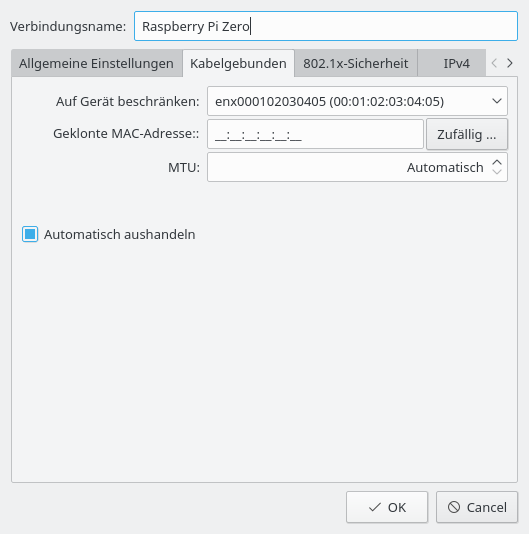
\includegraphics[scale=0.42]{images/OTG_Pi_Verbindungsname.png}
	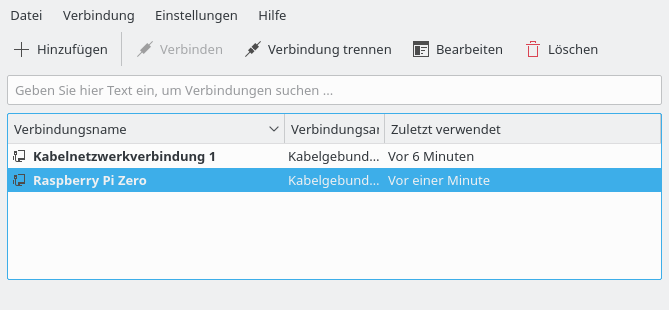
\includegraphics[scale=0.42]{images/OTG_Netzwerkverbindungen.png}
%	\caption{}
  \label{OTG_LINUX_Netzwerkverbindungen}
\end{figure}


Nun kann bei den IPv4-Einstellungen die Methode "`Automatisch"' eingestellt werden.

%\begin{figure}[ht]
%  \centering
%  \includegraphics[scale=0.42]{images/OTG_NetzwerkverbindungenAutomatisch.png}
%	\caption{}
%  \label{OTG_LINUX_Netzwerkverbindungen}
%\end{figure}

\clearpage
%\input{OTG_Mint}





\section{SSH Verbindung (Linux)} 

Nach der Einrichtung kann per SSH-Client eine Verbindungen zum Raspberry Pi hergestellt werden. Dazu muss in einem Terminal folgender Befehl eingegeben werden:

\begin{console} 
	ssh -X pi@raspberrypi.local
\end{console}

Um grafische Programme am Host anzeigen zu k�nnen, muss der Parameter \texttt{-X} angegeben werden. "`\textbf{pi}"' ist der Standardbenutzer am System. Dann wird eine X-Server Verbindung via SSH hergestellt. Verbindet man sich zum ersten Mal mit dem Raspberry Pi, so wird noch eine Sicherheitswarnung ausgegeben. Der kryptographische Schl�ssel f�r die Verbindung ist dem lokalen System noch nicht bekannt.%  und muss best�tigt werden.
\begin{screensmall}
The authenticity of host 'raspberrypi.local (192.168.137.10)' can't be established.
ECDSA key fingerprint is SHA256:Dcf3HYgE2GHnNnZ8Xhv8iJ9yA+zvfXBC9COm2eL9i0w.
Are you sure you want to continue connecting (yes/no)? 
Warning: Permanently added 'raspberrypi.local,192.168.137.10' (ECDSA) to the list of known hosts.
\end{screensmall}

Die Frage muss mit \texttt{yes} best�tigt werden. Anschlie�end muss das Default-Passwort von Raspbian "`\textbf{raspberry}"' eingegeben werden. Nun sollte man den Raspberry Pi Prompt \texttt{pi@rasbperrypi:\textasciitilde  \$} sehen. 

Wechselt man zu einem anderen Raspberry Pi mit den gleichen Namen oder installiert das System nochmals, so kann es passieren, dass eine Fehlermeldung ausgegeben wird, weil sich der kryptographische Schl�ssel ge�ndert hat.

\begin{screensmall} 
@@@@@@@@@@@@@@@@@@@@@@@@@@@@@@@@@@@@@@@@@@@@@@@@@@@@@@@@@@@
@    WARNING: REMOTE HOST IDENTIFICATION HAS CHANGED!     @
@@@@@@@@@@@@@@@@@@@@@@@@@@@@@@@@@@@@@@@@@@@@@@@@@@@@@@@@@@@
\end{screensmall} 

%The ECDSA host key for raspberrypi.local has changed,
%and the key for the corresponding IP address 169.254.229.192
%is unknown. This could either mean that
%DNS SPOOFING is happening or the IP address for the host
%and its host key have changed at the same time.
%@@@@@@@@@@@@@@@@@@@@@@@@@@@@@@@@@@@@@@@@@@@@@@@@@@@@@@@@@@@
%@    WARNING: REMOTE HOST IDENTIFICATION HAS CHANGED!     @
%@@@@@@@@@@@@@@@@@@@@@@@@@@@@@@@@@@@@@@@@@@@@@@@@@@@@@@@@@@@
%IT IS POSSIBLE THAT SOMEONE IS DOING SOMETHING NASTY!
%Someone could be eavesdropping on you right now (man-in-the-middle attack)!
%It is also possible that a host key has just been changed.
%The fingerprint for the ECDSA key sent by the remote host is
%SHA256:Dcf2HYyE2GHnNpZ8Xhv8iJ9yj+zvfXBC9COm2eL9i0w.
%Please contact your system administrator.
%Add correct host key in /home/evil/.ssh/known_hosts to get rid of this message.
%Offending ECDSA key in /home/evil/.ssh/known_hosts:9
%remove with:
%ssh-keygen -f "/home/evil/.ssh/known_hosts" -R raspberrypi.local
%ECDSA host key for raspberrypi.local has changed and you have requested strict checking.

In diesem Fall muss man die Verbindung aus den bekannten Hosts l�schen. Hierf�r muss folgendes Kommando ausgef�hrt werden:

\begin{console} 
	ssh-keygen -R raspberrypi.local
\end{console}

Optional kann auch der Parameter \texttt{-o UserKnownHostsFile=/dev/null} beim ssh-Befehl hinzugef�gt werden. Dann erfolgt keine �berpr�fung der Verbindung. 


\section{Einstellungen}


Als erstes kann das Raspberry Pi Software Configuration Tool (raspi-config)  gestartet werden. Dazu verwendet man den Aufruf "`sudo raspi-config"'.\\
Der Men�punkt "`Change User Password"' �ndert das Passwort f�r den Benutzer "`pi"'.\\
Danach sollte man die Regionseinstellungen mit dem Men�punkt "`Localisation Options"' einstellen. Im folgenden Untermen� kann man mit "`Change Locale"' die Sprache und Zeichensatz des Systems setzen. Hier w�hlt man z.~B. "`de\_AT.UTF-8 UTF8"' f�r �sterreich oder "`de\_DE.UTF-8 UTF8"' f�r Deutschland. "`en\_GB.UTF-8 UTF8"' und  "`C.UTF-8"' sind bereits ausgew�hlt und k�nnen zus�tzlich aktiv sein. Im n�chsten Fenster kann man dann die Sprache "`de\_AT.UTF-8 UTF8"' bzw. "`de\_DE.UTF-8 UTF8"' als Standardeinstellung �bernehmen.\\ 
Nun kann man mit "`Change Timezone"' die aktuelle Zeitzone ausw�hlen. F�r das geografische Gebiet kann man "`Europe"' ausw�hlen. Danach kann man als Zeitzone die Stadt "`Vienna"' oder "`Berlin"' ausw�hlen.\\
Bei der dritten Einstellung "`Change Keyboard Layout"' kann man das Tastatur-Layout aktualisieren.
%ausw�hlen:\\
%Keyboard model: Generic 105-key (Intl) PC \textit{(Tastatur mit Windows Taste)}\\
%Keyboard layout: Other\\
%Country of origin for the keyboard: German\\
%Keyboard layout: German - German (eliminate dead keys)\\
%Key to function as AltGr: The default for the keyboard layout\\
%Compose key: No compose key\\
%Use Control+Alt+Backspace to terminate the X server?: <Yes>\\


\clearpage
\section{Aktualisierungen und Programme}


%\textbf{Raspberry Pi:}
\begin{console}
sudo -i
apt-get update && apt-get -y upgrade
apt-get clean
apt-get install mono-complete
apt-get clean
apt-get install python-dev python-openssl rpi.gpio
apt-get clean
apt-get install python3-dev python3-openssl python3-rpi.gpio python3-gpiozero python3-pip
apt-get clean
apt-get install geany vim wiringpi pigpio git build-essential automake
apt-get clean
apt-get install minicom screen
apt-get clean

cd ~
mkdir Projekte
cd ~/Projekte

git clone https://github.com/mstroh76/TM1637Display
cd TM1637Display
g++ -o TM1637Display *.cpp -lwiringPi
cd ..
git clone https://github.com/mstroh76/Sensors-WiringPi.git
cd Sensors-WiringPi/DHT
g++ -o DHT main.cpp DHT.cpp -lwiringPi
cd ../HC-SR04
g++ -o HC-SR04 main.cpp HC-SR04.cpp -lwiringPi

cd ~/Projekte
wget https://goo.gl/isrNeJ
git clone https://github.com/chirndler/wiringpi.net.sensors.git
cd wiringpi.net.sensors
xbuild /p:Configuration=Release wiringpi.net.sensors.sln

cd ~/Projekte
pip3 install wiringpi
git clone https://github.com/depklyon/raspberrypi-python-tm1637.git
cd raspberrypi-python-tm1637
python3 setup.py install
cd ..
git clone https://github.com/jdupl/dhtxx-rpi-python3.git
cp dhtxx-rpi-python3/dhtxx.py /usr/local/lib/python3.5/dist-packages/

reboot
\end{console}



\chapter*{Anhang}


\section*{Lizenz}
\lhead{}
\chead{}
\rhead{ANHANG}

\begin{figure}[ht]
  \centering
  
\includegraphics[scale=1.0]{images/by-sa.png}
\end{figure}

Dieses Werk steht unter der Lizenz Creative Commons BY-SA 3.0 (\url{https://creativecommons.org/licenses/by-sa/3.0/at}). Sie erlaubt ausdr�cklich, das Werk zu vervielf�ltigen, zu verbreiten und �ffentlich zug�nglich machen. Es ist weiters erlaubt diese Werk zu ver�ndern und darauf aufbauen zu erweitern. Es muss allerdings der Urheber genannt werden und die aufbauende Arbeit muss unter der gleichen Lizenz stehen.\\
Die Anleitung enth�lt Teile aus anderen E-Book's des Autors Martin Strohmayer, diese k�nnen �ber\\
Amazon \urlsmall{https://www.amazon.de/-/e/B071HJ6GYJ} und\\
Google \urlsmall{https://play.google.com/store/books/author?id=Martin+Strohmayer}\\
bezogen werden.\\
Wenn sie die Arbeit des Autors unterst�tzen wollen erwerben Sie das E-Book, Danke!\\

Es wurden freie (CC0) Grafiken von Openclipart verwendet \url{https://openclipart.org}.\\ 
Schaltpl�ne und Ansichten Steckplatine wurden mit Fritzing erstellt \url{http://fritzing.org}.
%DHT22, 
Es wurden Fritzing Componenten von Adafruit  \url{https://github.com/adafruit/Fritzing-Library} und 
% HC-SR04
Ricky Ng-Adam %\url{https://github.com/rngadam/ART/tree/master/ele/fritzing} 
und
% Grove
Yihui Xiong \url{https://github.com/mcauser/seeed-fritzing-parts}
 verwendet. Sie werden ebenfalls unter der CC-BY-SA Lizenz zur Verf�gung gestellt. 


\subsection*{Haftungsausschluss}

Die Benutzung dieses Buches und die Umsetzung der darin enthaltenen Informationen erfolgt ausdr�cklich auf eigenes Risiko. Haftungsanspr�che gegen den Verlag und den Autor f�r Sch�den materieller oder ideeller Art, die durch die Nutzung oder Nichtnutzung der Informationen bzw. durch die Nutzung fehlerhafter und/oder unvollst�ndiger Informationen verursacht wurden, sind grunds�tzlich ausgeschlossen. Rechts- und Schadensersatzanspr�che sind daher ausgeschlossen. Das Werk inklusive aller Inhalte wurde unter gr��ter Sorgfalt erarbeitet. Der Verlag und der Autor �bernimmt jedoch keine Gew�hr f�r die Aktualit�t, Korrektheit, Vollst�ndigkeit und Qualit�t der bereitgestellten Informationen. Druckfehler und Falschinformationen k�nnen nicht vollst�ndig ausgeschlossen werden. F�r die Inhalte, der in diesem Buch abgedruckten Internetseiten, sind ausschlie�lich die Betreiber der jeweiligen Internetseiten verantwortlich. Der Verlag und der Autor haben keinen Einfluss auf Gestaltung und Inhalte fremder Internetseiten. Verlag und Autor distanzieren sich daher von allen fremden Inhalten. %Zum Zeitpunkt der Verwendung waren keinerlei illegalen Inhalte auf den Webseiten bekannt.



\end{document}
%EOF
